\section{Evaluation}
We conducted two user-centered evaluations: the first one is to investigate how SensePath is used by a domain expert, and the second one is to discover whether SensePath has any potential advantages compared with a traditional method. We first conducted a number of user studies of participants carrying out an online sensemaking task to establish a ground truth dataset. Then, we recruited HCI researchers to analyze the sensemaking processes of these participants. In this section, we regard these HCI researchers as ``analysts'' and people performing sensemaking tasks as ``participants'' or ``sensemakers''.

We recruited two participants to take part in this study: a post-doctoral researcher and a PhD student, both males. Participants were given the same task, which was to use the Chrome browser to find appropriate accommodation for two academics attending a conference at the World Bank headquarters in Washington, D.C. We provided participants with information about the location and dates of the conference, but gave no further details in the scenario to maintain suitable complexity in the task, and to ensure it was as realistic as possible.

Both participants were given 30 minutes to perform the task. Throughout the study, their sensemaking actions were collected within SensePath, and their screens were also recorded. We also encouraged participants to think aloud throughout the study, and finally conducted a semi-structured interview asking them to reveal:

\begin{itemize}
	\item The rationale behind their choice
	\item The strategy in approaching the task
	\item The process they went through in executing that strategy
\end{itemize}

\pagebreak

\subsection{Evaluation 1}

\subsubsection{Design}
The goal of this evaluation is to explore how SensePath is used by a domain expert performing a real-world task. We recruited an analyst with seven years of experience in qualitative research to analyze the actions captured in the sensemaking process outlined earlier using SensePath. We gave the analyst a short tutorial to introduce and explain features of SensePath, before practicing with a trial task. She was provided with a laptop running SensePath, connected to an external monitor, providing a multi-screen setup as in \autoref{fig:sp-evaluation-setup}. During the analysis, we encouraged the analyst to provide feedback through a think-aloud protocol. We recorded her responses and other observations using written notes. At the end of the analysis, we asked the analyst to complete a discovery sheet reporting her findings. A semi-structured interview was followed up to gain deeper understanding of her experience. The discovery sheet included the following sub-tasks:
\begin{itemize}
	\item Identify the sensemaker's strategy in approaching the task and characteristics demonstrating that.
	\item Identify the steps the sensemaker took in choosing suitable accommodation and provide a name (code/theme) for each step.
	\item Identify any interesting patterns in the data.
\end{itemize}

\begin{figure}
\centering
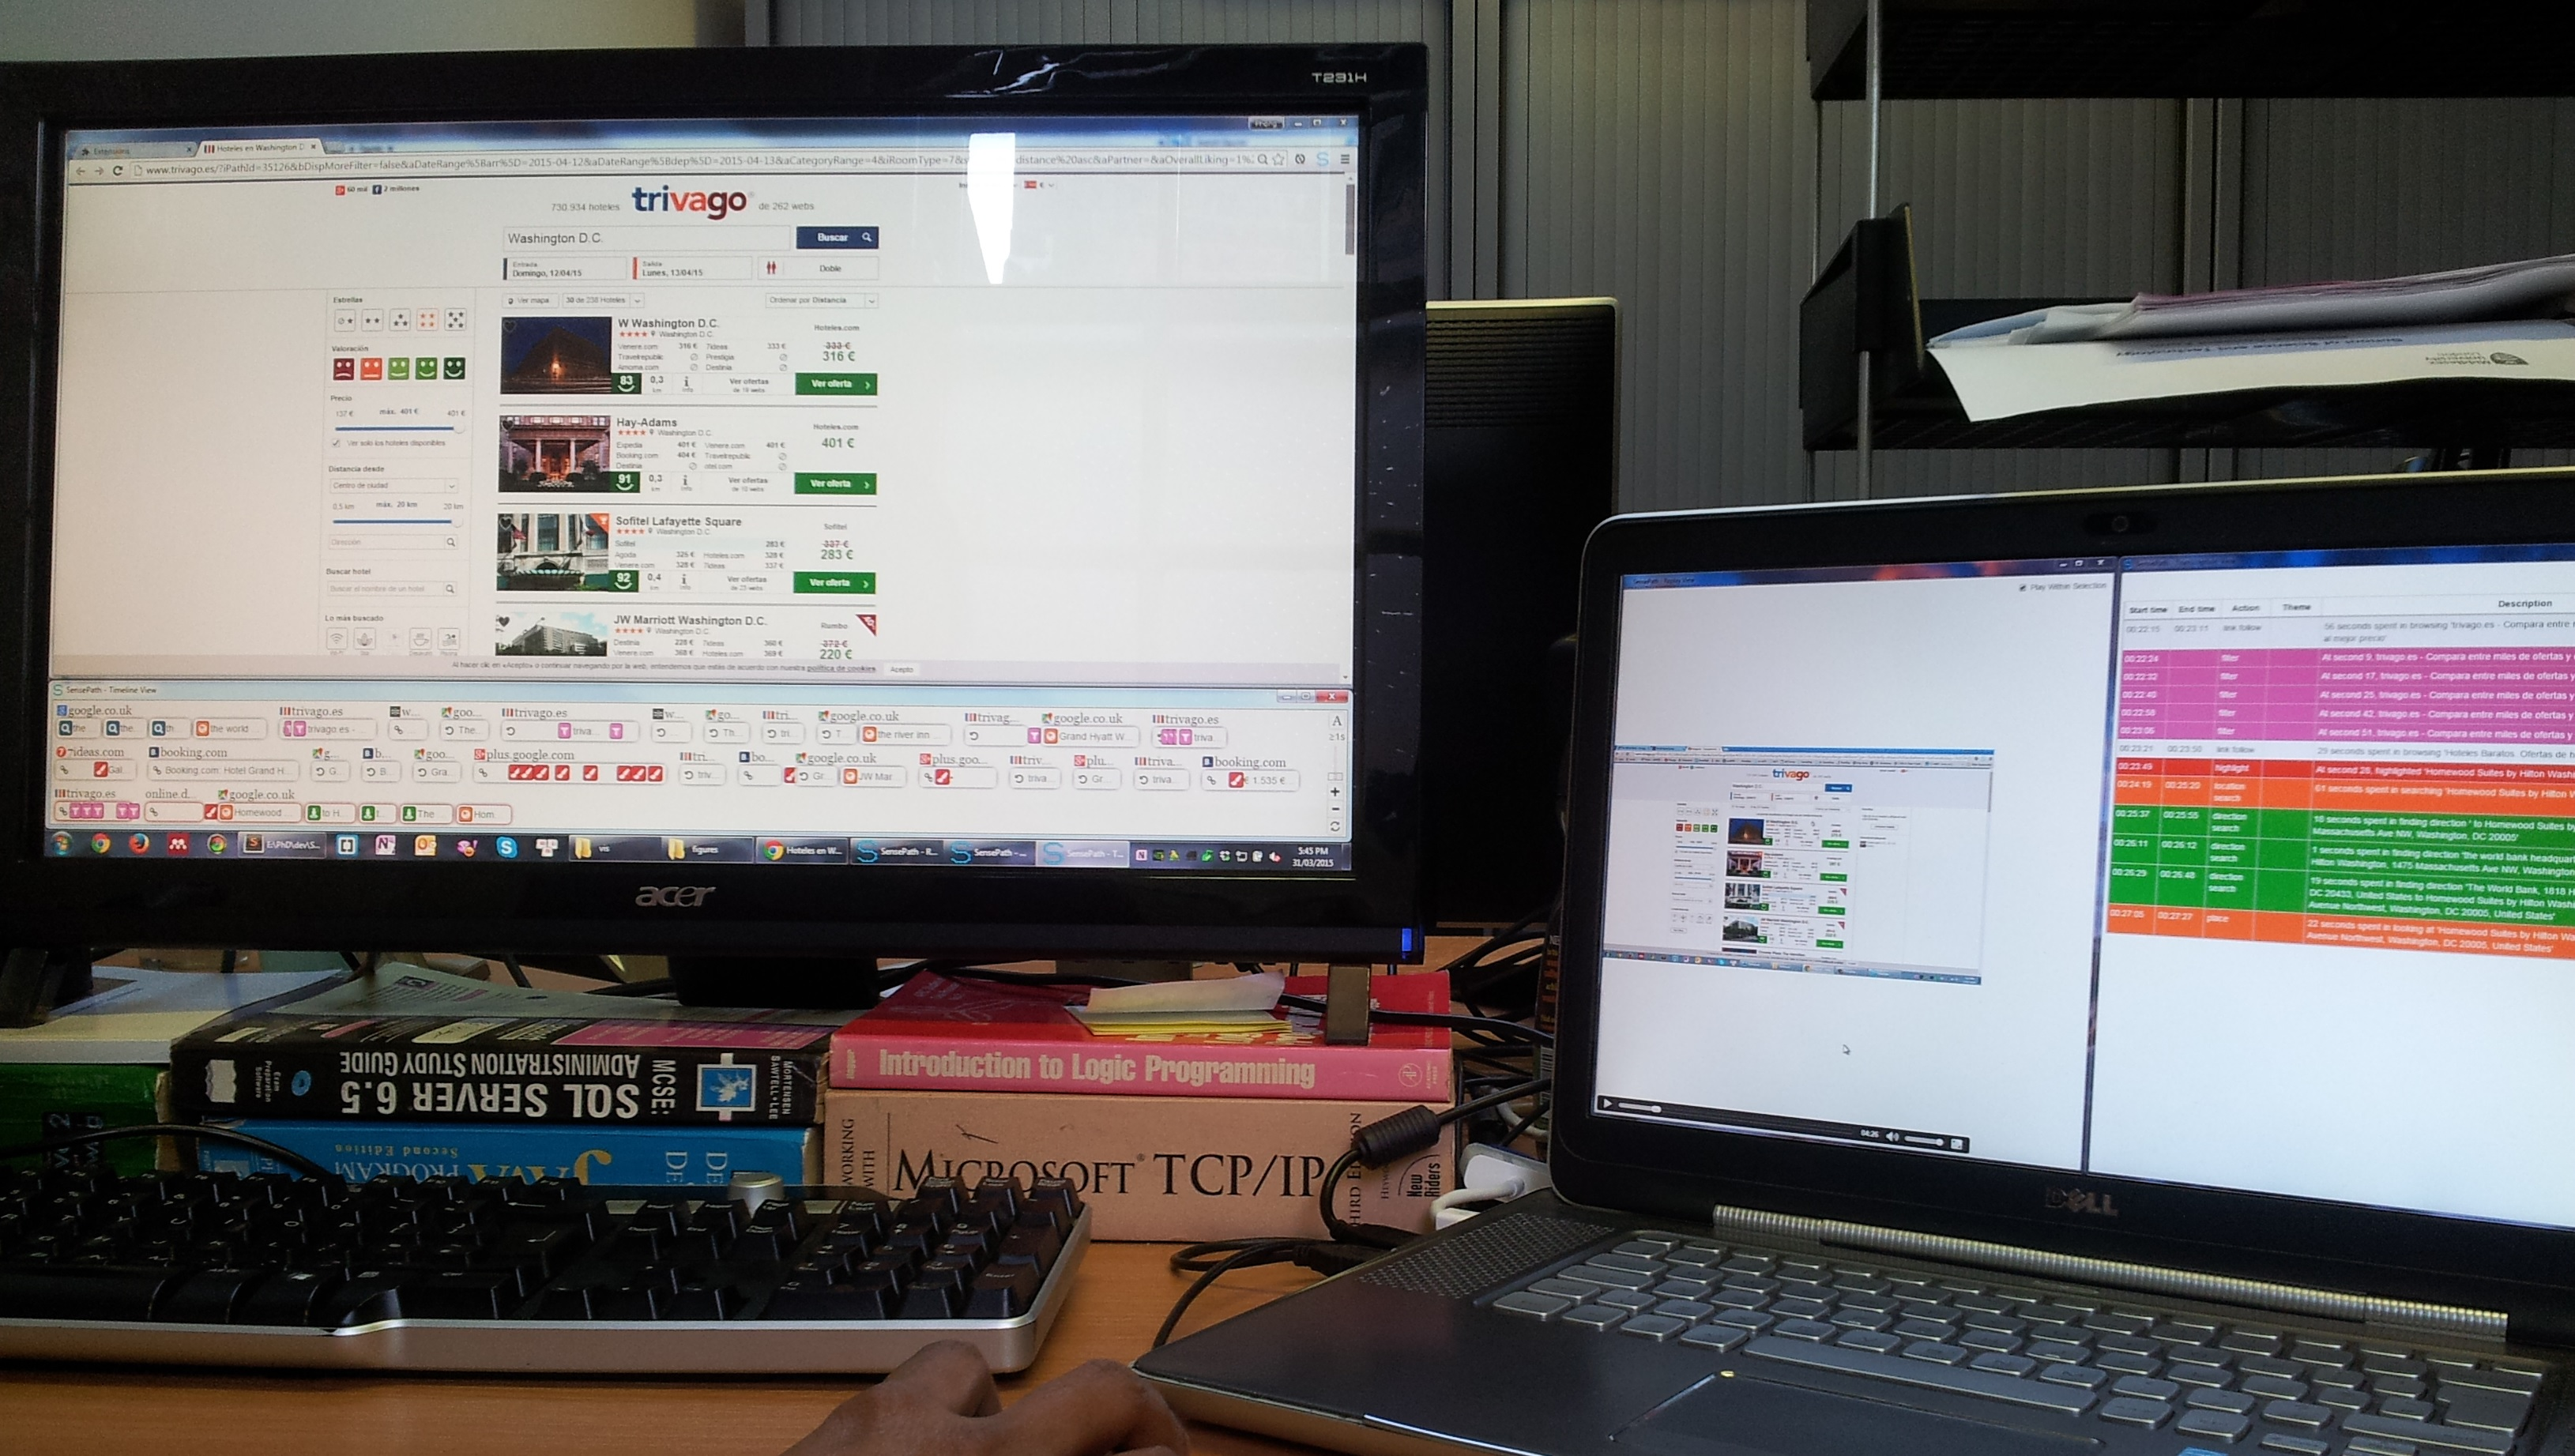
\includegraphics[width=\linewidth]{experiment-setup}
\caption[The setup of the qualitative analysis with SensePath]{The setup of the qualitative analysis with SensePath. The monitor on the left shows the timeline and browser views, and the laptop on the right shows the replay and transcription views.}
\label{fig:sp-evaluation-setup}
\end{figure}

\subsubsection{Findings}
The analyst took approximately one hour to analyze 30 minutes of study data. This shows a reduction of half the time taken using SensePath compared with traditional methods of video analysis, which would typically take around four hours of analysis for every hour of study data~\cite{Burr2006}.

The analyst initially used the timeline to view sensemaking actions at a low resolution, before focusing on interesting parts of the data in more detail. Because these actions are visualized in a single view, the analyst reported she could quickly make an initial summary assessment of the sensemaker's overall performance of the task, before identifying potentially interesting behaviors in the data. One such example of this is when she saw many highlights on a Google Plus page, next to each other in the timeline, she said ``It seems that the guy [the sensemaker] found interesting information on that [Google Plus] page because he highlighted a lot there''. She then moved the mouse over these highlight icons to read the highlighted text shown in the tooltips. Interestingly, she quickly concluded that ``He only focused on negative reviews''. She clicked on some of those icons to open up the Google Plus page to gain more context. Unfortunately, that page is content-dynamic, thus some highlighted texts failed to be reselected. She switched to watch the video in the replay view and heard that the participant was talking to us about his preference to negative reviews (we used think-aloud protocol), which confirmed her initial judgment. She also mentioned that offering a highlight feature to the sensemakers is useful because it enables her to quickly identify their interests.

To understand the whole sensemaking process, the analyst quickly went through all the actions shown in the timeline. The analyst was able to successfully describe the steps taken by the sensemakers in approaching to the task. We confirmed those steps were all correct by re-watching the capture video and verifying with the sensemakers. \autoref{fig:sp-evaluation-diagram} shows a reproduction of a written diagram created by the analyst illustrating the steps she identified. She explained the diagram to us; for instance, ``that guy searched for the address of the headquarters, then viewed it in Google Maps to get a sense of where it is''.

\begin{figure}
\centering
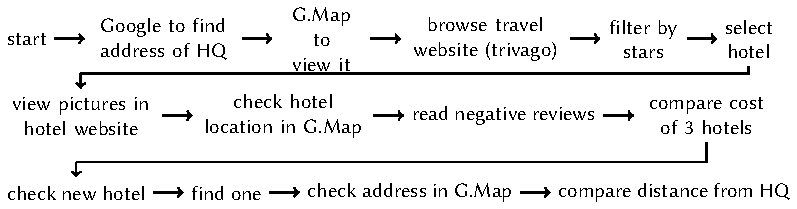
\includegraphics[width=\linewidth]{diagram}
\caption[Sensemaking steps]{Sensemaking steps. A reproduction of diagram written by the analyst during the evaluation illustrating the steps taken by the sensemaker in the task.}
\label{fig:sp-evaluation-diagram}
\end{figure}

The analyst reported that using the timeline view she could easily identify interesting recurring patterns because all actions are shown together. As an example for such patterns, when the sensemaker found a hotel in a booking website, he looked at its pictures first, then searched for its location in Google Maps, and checked its route to the headquarters. The sensemaker repeated this process for several hotels he found.

The analyst managed to find an overall strategy that the sensemaker applied in approaching the task: he targeted reasonably cheap hotels (evidenced by filtering out 5-star ones) and considered hotels close to the headquarters (supported by putting them in Google Maps for comparison). This confirmed with what the sensemaker told us: as a professional academic, he wanted to save money for the university, but also did not want to stay too far away from the conference venue.

The analyst commented that the video and audio recordings were intrinsic to carry out a fuller, more detailed analysis by providing additional information that was unavailable in the timeline and the browser views such as mouse movement or page scroll interactions. Therefore, the replay view helped her gain further insight into the sensemaker's behaviors. Because the analyst did not have to watch the whole video, she thought that she could save valuable time in the analysis. Moreover, she stated that as clicking on an action in the timeline view skipped to the relevant place in the screen capture, further time was saved in scrubbing through the video, which often happened in her experience of analyzing video data. For example, when seeing a long search action bar, she knew that the sensemaker spent much time in Google Maps, searching for a specific location; however, what exactly he was doing is neither available in the timeline nor the browser view. Thus, she needed to watch the video to get more information.

\subsection{Evaluation 2}

\subsubsection{Design}
The goal of this evaluation is to establish an initial understanding of whether SensePath has any advantages compared with a traditional method. We conducted an experiment with two senior HCI researchers to analyze a short 15-minute video (part of the video used in the first evaluation) using thematic analysis, but only for the first two stages: transcription and coding, which SensePath is designed to support. One analyst used SensePath and the other used a transcription software called \textit{Transcription} ~\footnote{\url{https://code.google.com/p/transcriptions/}}. This tool shows the transcribing video and a text editor side by side, and provides a set of shortcuts for quick video manipulation such as pause/play or step forward/backward. This enables users to control the video play while focusing on the editor to type in the transcript, thus accelerates the transcription. The experiment setup and procedure were the same as in the first evaluation. The analysts were asked to produce a transcript of the video, identify the steps the sensemaker took in performing the task, and assign codes for them. Timing for each analysis stage was recorded, and an interview was followed after the analysis to gain deeper understanding of their processes.

\subsubsection{Findings}
The result showed that SensePath can significantly reduce time for transcription. In the baseline condition, it took the analyst 60 minutes to transcribe the video, about 15 minutes of them spent for the think-aloud audio. In SensePath condition, transcribing was done automatically using the captured actions, and it took the analyst 5 minutes to traverse all actions in the timeline to get a sense of the sensemaker's process.

In regard to accuracy, SensePath identified 39 actions and all are correct (each action is verified by us). In the baseline condition, the analyst identified additional actions that SensePath was unable to capture because the browser did not reload such as ``click on a pull-down menu to see more options'' or ``encircle the rating point with mouse movement''. However, he missed two actions that were correctly identified by SensePath: ``set checkin and checkout date'' and ``change sorting criteria''.

Watching the video helped the analyst transcribe with richer information. For instance, SensePath can only record where a web page came from such as manually typing the address or linking from another page. Whereas in the baseline condition, more context can be added such as which button was clicked to open that new page. However, SensePath can save time from transcribing long text such as for highlights or annotations.

For coding, in the baseline condition, the analyst copied the transcript to Excel and assigned codes in a column next to the text. The analyst using SensePath can directly assigned codes to actions in the timeline view. SensePath was only slightly faster than the traditional method (40 minutes vs. 45 minutes). It could because the analyst using SensePath needed to familiarize himself with the data by watching some parts of the video a few times, whereas the other analyst already spent a long time watching the video during the transcription stage.

In both conditions, the analysts produced reasonable and comparable codes for the steps they identified. For example, in the baseline condition, the analyst created codes such as ``Google search for location'', ``drill down'', ``assessment'' and ``assessing relevance of evidence''. The analyst with SensePath produced similar codes including ``looking for headquarters location'', ``locate option'', ``assess proximity'', ``assess price'' and ``assess reviews''.

Similar to the analyst in the first evaluation, the analyst with SensePath also quickly went through all sensemaking actions to obtain an overview of the process, before drilling down to actions of interest. Especially, the analyst often used actions in the timeline as a navigation to the part of the video he wanted to watch. He said he needed to watch some parts of the video several times to understand the intention of the sensemaker, and clicking on the actions enables him to quickly go to the correct part.